\section{Evaluation plan}
\label{sec:eval}

\begin{table*}[tbh]
\begin{tabular}{|l|c|c|}
\hline & Palm Pre Cortex-A8 256MB RAM & Android ARM 1136-JS 128MB RAM \\ 
\hline Basic ARM kernel & $52$ & $154$ \\ [2pt]
 Debian ARM Lenny & $1186$ & Crashes during boot \\ [2pt]
 TTY-Linux-i486 & $>2000$ & Unable to get x86 guest mode qemu to run on arm \\[2pt]
\hline 
\end{tabular}
\caption{
Virtualization Results: Kernel Boot time in seconds
}
\label{tab:virt_results}
\end{table*}

\subsection{Preliminary Virtualization Results}

Currently, we have evaluated the overhead of virtualization with a QEMU-based implementations running various distributions of Linux on both the Android and the Palm Pre as shown in Table \ref{tab:virt_results}. The most successful implementation used ARM on ARM virtualization and a basic ARM kernel image provided along with QEMU. Unfortunately, even this implementation was far too slow, taking 52 seconds to boot on the Pre and 154 seconds to boot on the Android. Additionally response times were terrible, often taking several seconds to display text input. A Debian ARM Lenny image took over 15 minutes to boot on the Palm Pre and crashed on the Android during boot. x86 emulation on ARM was also tested, with a TTY-Linux image; however, this was the slowest by far, taking over half an hour to boot on the Palm Pre. On the Android, x86 guest mode QEMU would not even run. Overall these experiments suggest that binary translation is not usable and that we need to explore for different virtualization techniques listed in Section \ref{sec:design}.

\subsection{X-Server numbers}

An important part of our system is the X server to visualize and interact with the applications.  While our current design is somewhat limited in that it has too many layers of abstractions (using SDL as the backend), we've taken efforts to make the server run faster, which resulted in a much better user experience.  The biggest  performance improvement was moving from basic SDL to SDL-GLESv2 which improved the ``feel'' of X and the applications inside of it noticeably.  To try to capture this speed improvement we ran x11perf, which helps quantify the performance improvements.  As shown in Table \ref{tab:x_results}, there was noticeable improvements in a number of tests.
These tests we run from a Debian chroot, using localhost communication (not domain sockets) with the server, on the Palm Pre.  The tests were arbitrarily selected, with an attempt at finding representative ones.  These numbers should only be taken as illustrating the general performance improvements, not as an accurate measure of what real applications will be like.

\begin{table}[ht]
{\small
\hfill{}
\begin{tabular}{|l|c|c|c|}
\hline Benchmark & Xsdl & Xsdl-gles & \%Speedup \\ [2pt] 
\hline oddtilerect$100$ & $9950$ & $11500$ & $15.57\%$ \\ [2pt]
scroll$100$ & $6680$ & $7700$ & $15.26\%$ \\ [2pt]
copy$100$ & $2940$ & $3440$ & $17.01\%$ \\ [2pt]
rect$100$ & $15700$ & $18900$ & $20.38\%$ \\ [2pt]
fcircle$100$ & $8130$ & $9940$ & $22.26\%$ \\ [2pt]
ftext & $481000$ & $556000$ & $11.43\%$ \\ [2pt]
\hline 
\end{tabular}}
\hfill{}
\caption{ X server rendering with x11perf }
\label{tab:x_results}
\end{table}

\begin{figure}[tbh]
\centering
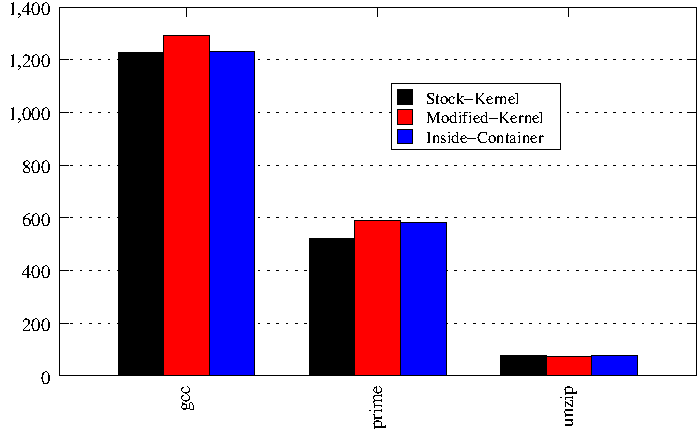
\includegraphics[width=1.0\columnwidth]{perf}
\caption{Running time comparison}
\label{fig:perf}
\end{figure}

\subsection{LXC Performance numbers}

Our addition of the linux container functionality to the kernel imposed no noticeable overhead to the phone.  Our testing (\ref{sec:lxc_perf}) proved that i/o, cpu, and memory performance was unaffected by the addition of the container code.  There was no overhead to running inside a container as well.

\begin{table}[ht]
{\small
\hfill{}
\begin{tabular}{|l|c|c|c|}
\hline
\multirow{3}{12mm}{Benchmark}    & \multirow{3}{12mm}{Stock\\Kernel} & \multirow{3}{12mm}{Modified\\Kernel} & \multirow{3}{12mm}{Inside a\\Container} \\
&&&\\
&&&\\
\hline
gcc-apache   & $1229$s      & $1293$s          & $1232$s            \\
prime number & $522$s       & $590$s           & $581$s             \\
unzip        & $76$s        & $73.44$s         & $76.29$s           \\
\hline 
\end{tabular}}
\hfill{}
\caption{ Peformance benchmarks on Linux Containers }
\label{tab:lxc_perf}
\end{table}

\subsection{Future Evaluation}

Our goal for this project is to integrate an isolation technique which is usable and is integrated with the mobile device. We propose to evaluate the overhead due to the isolation framework and also ensure correctness using standard benchmarks. In particular, we plan to evaluate the latency involved in running an interactive application and measure how much benefit is obtained due to the shared X server running natively. We also plan to profile the memory and cpu usage overhead entailed by our design and compare the same with the application running natively. The VM Controller will be integrated with the window manager of at least one mobile device and we will demonstrate the ability to start and stop applications using the controller.
